\section{Primary Evaluation: The Base Paper's 19 Real Hospitals (PCa-19)}
\label{sec:pca19}
This section evaluates the full DP-FPS framework on the exact patient-level data of the base paper. Unlike TCGA-PRAD, PCa-19 has real, independently collected hospitals, a pre-biopsy prediction task with PSA and MRI, and enough countries for external validation.

\subsection{Reproduction of the Authors' Protocol}
\label{sec:p19_repro}
We first re-implemented the authors' public protocol line by line: scikit-learn logistic regression on the raw Ettala and Noh variables, a stratified 80/20 split per hospital, one-shot FedAvg (a sample-size-weighted average of fully trained local models), and free-riding evaluated on 100\% of the excluded hospital. Monte-Carlo random states are drawn exactly as in their scripts. Running the authors' own code and our re-implementation with the same seed gives identical matrices for both calculators (validation check in Section~\ref{sec:threats_validity}). Table~\ref{tab:pca19_repro} confirms the base paper's qualitative findings: the published Noh calculator is almost as good as centralised training (AV \pRepNohBL{} vs \pRepNohCEN{}), the Ettala architecture is weaker, and FL, FR and CEN are within a few thousandths of each other.

\begin{table}[t]
\caption{Reproduction of the base paper's protocol on PCa-19 (50 Monte-Carlo repeats; AV = mean over hospitals, AVW = patient-weighted). Our re-implementation gives the same numbers as the authors' code (Section~\ref{sec:p19_repro}).}
\centering\footnotesize
\begin{tabular}{lcccc}
\toprule
& \multicolumn{2}{c}{Noh variables} & \multicolumn{2}{c}{Ettala variables} \\
Strategy & AV & AVW & AV & AVW \\
\midrule
Published calculator (BL) & 0.827 & 0.847 & 0.792 & 0.830 \\
Local (LOC) & 0.818 & 0.847 & 0.799 & 0.847 \\
Centralised (CEN) & 0.827 & 0.849 & 0.813 & 0.852 \\
One-shot FedAvg (FL) & 0.826 & 0.848 & 0.803 & 0.843 \\
Free-rider (FR) & 0.827 & 0.847 & 0.803 & 0.840 \\
\bottomrule
\end{tabular}
\label{tab:pca19_repro}
\end{table}


\subsection{Training Strategies under the DP-FPS Protocol}
Under our protocol (standardised log-PSA, log-volume, age and PI-RADS indicators; iterative FedAvg/FedProx with $T=20$, $E=5$; 20 seeds), the sustainability result of the base paper holds on its own data (Fig.~\ref{fig:pca19_strategies}). Joining the federation gives no significant average gain over local training (FL$-$LOC $=\pDFLminusLOC$). A free-rider obtains almost the same model (FR$-$FL $=\pDFRminusFL$), and federated training matches pooled training (CEN$-$FL $=\pDCENminusFL$). Per hospital, \pGainSig{} hospitals gain significantly from joining and \pLossSig{} lose. The free-rider learning curve rises from \pLcFrOne{} with one contributing hospital to \pLcFrFive{} with five and then flattens (\pLcFrLast{} with 18), so a small consortium suffices, as the base paper argued.

One negative result must be reported. The published Noh calculator, trained in Korea without any federation, is not beaten on the hospital-averaged AUC (FL$-$Noh $=\pDFLminusNoh$). The gap is driven by the two smallest Spanish hospitals (16 and 79 patients). On the patient-weighted AUC, FL is ahead (\pWFL{} vs \pWNoh{}). FL clearly outperforms the Ettala architecture (FL$-$Ettala $=\pDFLminusEtt$).

\begin{figure}[!t]
\centering
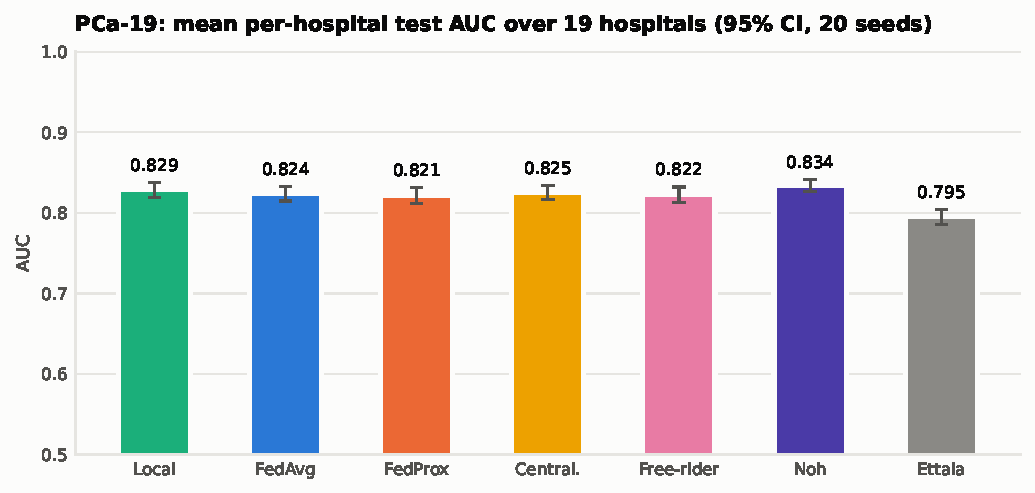
\includegraphics[width=\columnwidth]{figures/figure14_pca19_strategies.pdf}
\caption{PCa-19: mean per-hospital test AUC of each strategy over the 19 real hospitals (20 seeds, 95\% CI).}
\label{fig:pca19_strategies}
\end{figure}

\subsection{External Validation and Calibration}
The base paper evaluates only within its hospital set. We add \emph{leave-one-country-out} validation: models are trained on seven countries and tested on all patients of the eighth (Table~\ref{tab:pca19_loco}); preprocessing statistics never include the held-out country. Treating the eight countries as independent external tests, federated training matches centralised training (FedAvg$-$CEN $=\pLocoAvgCen$) and the published Noh calculator (FedAvg$-$Noh $=\pLocoAvgNoh$). DP at $\varepsilon=5$ costs a small but significant $\pLocoDpFive$ AUC.

Discrimination transports across countries; calibration does not. Observed/expected ratios of the FedAvg model range from \pOeMin{} to \pOeMax{} across countries, reflecting different csPCa prevalence (12--47\%). DP adds a second, previously unreported problem: it makes predictions too extreme. The mean calibration slope is $\pSlopeNoDP$ without DP but $\pSlopeDpFive$ at $\varepsilon=5$ and $\pSlopeDpOne$ at $\varepsilon=1$; the last two intervals exclude 1. A simple fix is \emph{local recalibration} on 20\% of a new country's patients (Table~\ref{tab:pca19_recal}, Fig.~\ref{fig:pca19_recal}). Re-estimating only the intercept reduces $|\log \mathrm{O/E}|$ from \pRecalOeRaw{} to \pRecalOeInt{} (paired difference $\pRecalOeDiff$). Re-estimating intercept and slope restores the DP model's slope from \pRecalSlopeDpRaw{} to \pRecalSlopeDpLog{}. Neither step changes the AUC, and both use only a few dozen to a few hundred local patients. Decision-curve analysis (Fig.~\ref{fig:pca19_dca}) shows positive net benefit over biopsying all men for every federated model at thresholds of 10--40\%.

\begin{table*}[t]
\caption{Leave-one-country-out external validation on PCa-19: train on the other seven countries, test on all patients of the held-out country (mean of 20 seeds). O/E = observed/expected events; slope = calibration slope (ideal 1).}
\centering\small
\begin{tabular}{lrrccccccc}
\toprule
& & & \multicolumn{3}{c}{FedAvg} & \multicolumn{2}{c}{FedProx + DP ($\varepsilon=5$)} & \multicolumn{2}{c}{Noh (published)} \\
Country & $n$ & csPCa\% & AUC & O/E & slope & AUC & slope & AUC & O/E \\
\midrule
China & 842 & 31 & 0.872 & 0.78 & 1.08 & 0.851 & 0.81 & 0.874 & 0.97 \\
Germany & 925 & 43 & 0.842 & 1.01 & 1.07 & 0.844 & 0.79 & 0.833 & 1.12 \\
Italy & 218 & 12 & 0.821 & 0.47 & 0.89 & 0.819 & 0.67 & 0.825 & 0.54 \\
Netherlands & 266 & 26 & 0.904 & 0.83 & 1.30 & 0.877 & 1.00 & 0.934 & 1.03 \\
South Korea & 996 & 33 & 0.896 & 0.83 & 1.45 & 0.890 & 1.01 & 0.886 & 1.00 \\
Spain & 1640 & 46 & 0.825 & 1.24 & 0.93 & 0.820 & 0.72 & 0.819 & 1.31 \\
USA & 590 & 47 & 0.783 & 1.30 & 0.86 & 0.776 & 0.65 & 0.765 & 1.55 \\
United Kingdom & 133 & 29 & 0.905 & 0.78 & 1.10 & 0.903 & 0.83 & 0.907 & 0.88 \\
\bottomrule
\end{tabular}
\label{tab:pca19_loco}
\end{table*}

\begin{table}[t]
\caption{Local recalibration on 20\% of each held-out country, evaluated on the other 80\% (mean over 8 countries and 20 seeds). $|\log$ O/E$|$ = 0 and slope = 1 are ideal; DP rows are FedProx + DP.}
\centering\scriptsize
\setlength{\tabcolsep}{4pt}
\begin{tabular}{llccc}
\toprule
Model & Recalibration & $|\log$ O/E$|$ & Slope & Brier \\
\midrule
FedAvg & none & 0.263 & 1.09 & 0.145 \\
 & intercept & 0.071 & 1.09 & 0.136 \\
 & int.\,+\,slope & 0.074 & 0.99 & 0.138 \\
\midrule
DP $\varepsilon=5$ & none & 0.260 & 0.81 & 0.150 \\
 & intercept & 0.080 & 0.81 & 0.140 \\
 & int.\,+\,slope & 0.074 & 0.99 & 0.140 \\
\midrule
DP $\varepsilon=1$ & none & 0.263 & 0.80 & 0.151 \\
 & intercept & 0.081 & 0.80 & 0.140 \\
 & int.\,+\,slope & 0.074 & 1.00 & 0.140 \\
\midrule
Noh & none & 0.205 & 0.97 & 0.144 \\
 & intercept & 0.075 & 0.97 & 0.137 \\
 & int.\,+\,slope & 0.077 & 0.97 & 0.138 \\
\bottomrule
\end{tabular}
\label{tab:pca19_recal}
\end{table}


\begin{figure}[!t]
\centering
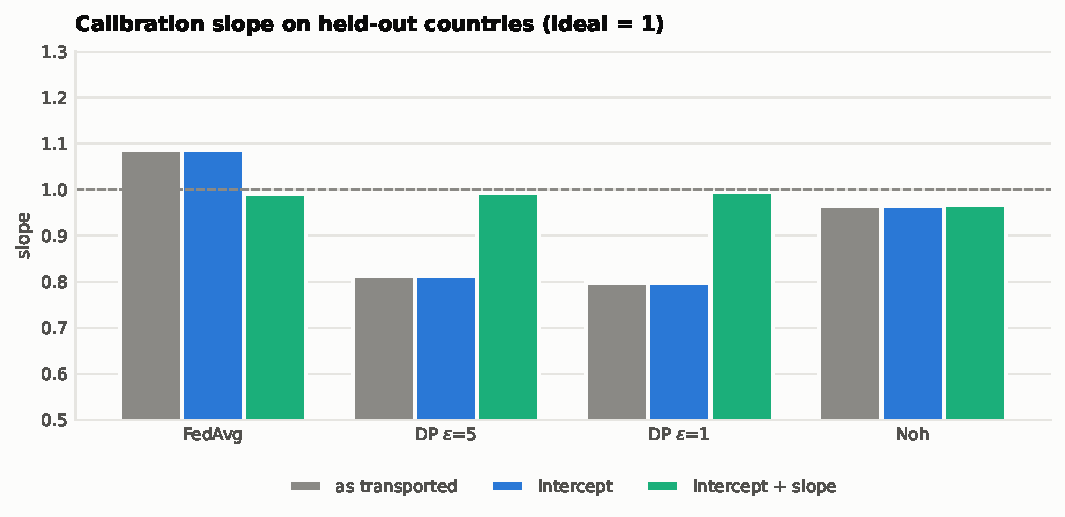
\includegraphics[width=\columnwidth]{figures/figure17_pca19_recalibration.pdf}
\caption{Calibration slope on held-out countries before and after local recalibration on 20\% of the country's patients.}
\label{fig:pca19_recal}
\end{figure}

\begin{figure}[!t]
\centering
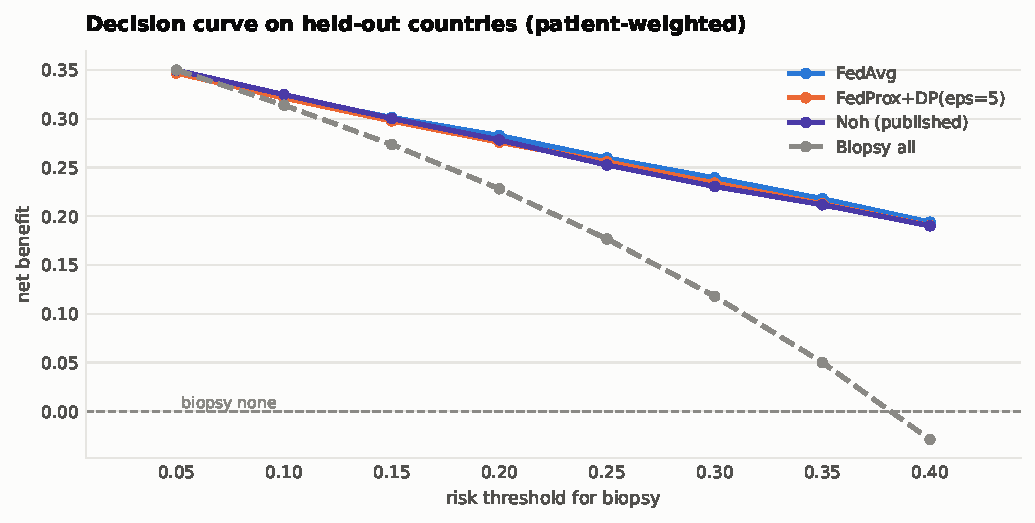
\includegraphics[width=\columnwidth]{figures/figure16_pca19_dca.pdf}
\caption{Decision curves on held-out countries (patient-weighted over the eight leave-one-country-out folds).}
\label{fig:pca19_dca}
\end{figure}

\subsection{Privacy and Drift on Real Hospitals}
Table~\ref{tab:pca19_privacy} and Fig.~\ref{fig:pca19_privacy} repeat the privacy grid on the real hospitals. With \pNineN{} patients, privacy is almost free. Even at $\varepsilon=0.5$ ($\sigma=\pSigmaHalf$) the mean per-hospital AUC changes by only $\pDpLossHalf$, compared with a loss of 0.06 at $\varepsilon=1$ on the 347-patient TCGA cohort. The utility cost of record-level DP is therefore governed mainly by the number of patients per hospital, not by $\varepsilon$ alone. FedProx reduces client drift by \pDriftRed\%, and DP noise inflates drift about tenfold at $\varepsilon=0.5$. At every privacy level, FedProx equals FedAvg with half the learning rate (largest mean difference \pProxHalfMax{} AUC). This confirms on real hospitals the step-size explanation found on TCGA.

\begin{table*}[t]
\caption{Privacy and drift on the 19 real hospitals (mean per-hospital test AUC, 20 seeds). The last two AUC columns are paired differences with 95\% CI; drift = mean $\|w_k-w^{t-1}\|$.}
\centering\small
\begin{tabular}{lccccccc}
\toprule
$\varepsilon$ & $\sigma$ & FedAvg & FedProx & FedAvg ($\eta/2$) & FedAvg $-$ no DP & FedProx $-$ FedAvg($\eta/2$) & Drift Avg / Prox \\
\midrule
no DP & -- & 0.824 & 0.821 & 0.821 & $--$ & $+0.000\ [\ensuremath{-}0.001, +0.002]$ & 0.33 / 0.23 \\
10 & 5.7 & 0.822 & 0.819 & 0.819 & $-0.002\ [\ensuremath{-}0.007, +0.003]$ & $+0.000\ [\ensuremath{-}0.001, +0.002]$ & 0.35 / 0.24 \\
5 & 10.5 & 0.822 & 0.819 & 0.819 & $-0.002\ [\ensuremath{-}0.007, +0.003]$ & $+0.000\ [\ensuremath{-}0.001, +0.002]$ & 0.48 / 0.33 \\
2 & 25.0 & 0.821 & 0.819 & 0.820 & $-0.003\ [\ensuremath{-}0.007, +0.001]$ & $-0.001\ [\ensuremath{-}0.003, +0.001]$ & 0.91 / 0.61 \\
1 & 49.0 & 0.820 & 0.819 & 0.819 & $-0.004\ [\ensuremath{-}0.008, +0.001]$ & $-0.001\ [\ensuremath{-}0.003, +0.002]$ & 1.69 / 1.13 \\
0.5 & 97.0 & 0.819 & 0.818 & 0.819 & $-0.005\ [\ensuremath{-}0.011, +0.001]$ & $-0.001\ [\ensuremath{-}0.003, +0.001]$ & 3.30 / 2.19 \\
\bottomrule
\end{tabular}
\label{tab:pca19_privacy}
\end{table*}


\begin{figure}[!t]
\centering
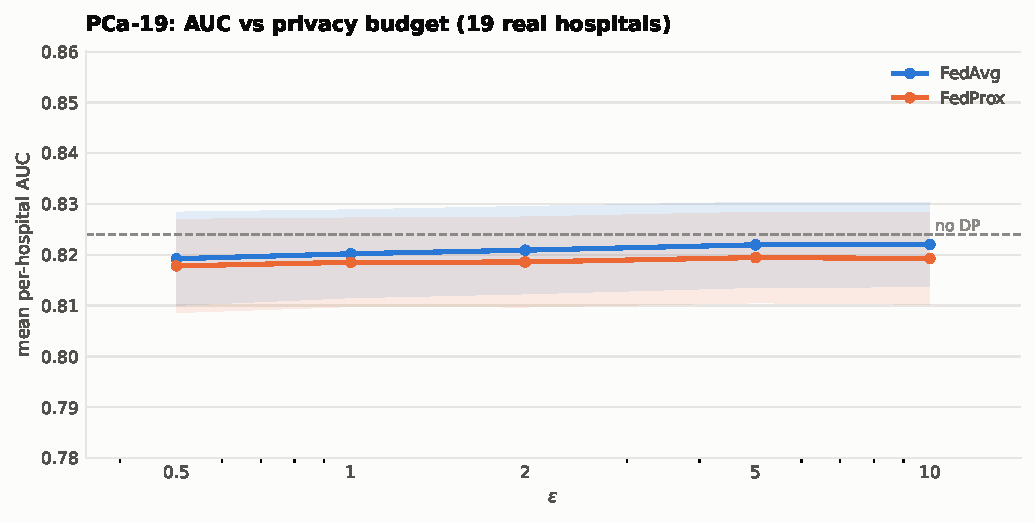
\includegraphics[width=\columnwidth]{figures/figure15_pca19_privacy.pdf}
\caption{PCa-19: mean per-hospital AUC vs privacy budget (20 seeds, 95\% CI); dashed line = no DP.}
\label{fig:pca19_privacy}
\end{figure}

\subsection{Stronger Baselines}
\label{sec:p19_baselines}
Table~\ref{tab:baselines} adds SCAFFOLD \cite{Karimireddy2020Scaffold}, FedAdam \cite{Reddi2021FedOpt}, a federated one-hidden-layer MLP, a converged FedAvg (400 instead of 100 local steps) and centralised non-linear references (histogram gradient boosting in the style of LightGBM \cite{Ke2017LightGBM}, random forest, MLP). FedNova \cite{Wang2020FedNova} normalises by the number of local steps and therefore equals FedAvg here, where every hospital runs the same number of steps. Hyper-parameters of the new baselines were tuned on four splits disjoint from the 20 evaluation splits. All federated variants lie within 0.006 AUC of FedAvg within hospitals: FedAdam $\blDAdam$, federated MLP $\blDMLP$, converged FedAvg $\blDLong$. SCAFFOLD removes \blScafDrift\% of client drift (FedProx: \blProxDrift\%) without changing AUC ($\blDScaf$). Under DP at $\varepsilon=1$ no variant improves on FedAvg (SCAFFOLD $\blDpScaf$, FedAdam $\blDpAdam$). Pooled non-linear models gain a little within the training hospitals (gradient boosting $\blDGB$) but not on unseen countries (gradient boosting $\blLGB$, federated MLP $\blLMLP$), where they are also less well calibrated. On TCGA with ten strongly skewed Dirichlet hospitals ($\alpha=0.1$) none of the alternatives beats FedAvg either (SCAFFOLD $\btScafLow$, FedAdam $\btAdamLow$, federated MLP $\btMLPLow$). With four pre-biopsy variables, the information in the data, not the model class or the federated optimiser, sets the ceiling; logistic regression is adequate and the best calibrated.

\begin{table*}[t]
\caption{Stronger baselines on PCa-19 (20 held-out seeds). Within-hospital: mean per-hospital test AUC over 19 hospitals. Leave-one-country-out: mean AUC over the 8 held-out countries and mean calibration slope; differences vs FedAvg are paired over countries ($n=8$). Last column: federated variants trained with DP at $\varepsilon=1$. FedNova equals FedAvg here (identical local steps at every hospital).}
\centering\small
\begin{tabular}{lcccccc}
\toprule
& \multicolumn{2}{c}{Within hospital} & \multicolumn{3}{c}{Leave-one-country-out} & DP \\
Model & AUC & $-$FedAvg [95\% CI] & AUC & $-$FedAvg [95\% CI] & Slope & $\varepsilon=1$ \\
\midrule
FedAvg & 0.816 & -- & 0.856 & -- & 1.08 & 0.811 \\
FedAvg (400 steps) & 0.818 & $+0.002\ [+0.001, +0.003]$ & 0.860 & $+0.004\ [\ensuremath{-}0.001, +0.009]$ & 1.02 & -- \\
FedProx & 0.811 & $-0.005\ [\ensuremath{-}0.008, \ensuremath{-}0.002]$ & 0.853 & $-0.003\ [\ensuremath{-}0.007, +0.000]$ & 1.12 & 0.809 \\
SCAFFOLD & 0.816 & $-0.000\ [\ensuremath{-}0.001, +0.000]$ & 0.856 & $+0.000\ [\ensuremath{-}0.001, +0.001]$ & 1.08 & 0.811 \\
FedAdam & 0.818 & $+0.002\ [+0.000, +0.005]$ & 0.861 & $+0.005\ [\ensuremath{-}0.003, +0.012]$ & 1.07 & 0.807 \\
Federated MLP & 0.821 & $+0.005\ [+0.001, +0.009]$ & 0.861 & $+0.005\ [\ensuremath{-}0.000, +0.010]$ & 0.92 & -- \\
\midrule
Central LR & 0.819 & $+0.003\ [+0.000, +0.005]$ & 0.860 & $+0.005\ [\ensuremath{-}0.002, +0.011]$ & 1.02 & -- \\
Central gradient boosting & 0.824 & $+0.009\ [+0.004, +0.014]$ & 0.853 & $-0.003\ [\ensuremath{-}0.011, +0.004]$ & 0.91 & -- \\
Central random forest & 0.820 & $+0.004\ [\ensuremath{-}0.002, +0.011]$ & 0.850 & $-0.006\ [\ensuremath{-}0.013, +0.001]$ & 0.95 & -- \\
Central MLP & 0.828 & $+0.012\ [+0.007, +0.017]$ & 0.861 & $+0.005\ [\ensuremath{-}0.001, +0.012]$ & 1.00 & -- \\
\bottomrule
\end{tabular}
\label{tab:baselines}
\end{table*}


\subsection{Sensitivity to Training Length}
Our default of $T=20$ rounds and $E=5$ local epochs (100 gradient steps) was chosen on TCGA and keeps the DP noise per step moderate. On PCa-19 it is slightly under-converged for some splits. Repeating the strategy comparison with 400 steps leaves every conclusion unchanged: FL$-$LOC $=\cvgFLminusLOC$, FR$-$FL $=\cvgFRminusFL$, CEN$-$FL $=\cvgCENminusFL$, and the published Noh calculator remains ahead on the hospital-averaged AUC (FL$-$Noh $=\cvgFLminusNoh$) but behind on the patient-weighted AUC (\cvgWFL{} vs \cvgWNoh{}).

\subsection{Personalisation}
Proximal fine-tuning helps exactly where expected. For the \pNSmall{} hospitals with fewer than 100 patients it improves on the global FedProx model by $\pPflSmall$ AUC, and over all hospitals by $\pPflAll$. For large hospitals ($\geq 400$ patients) it brings no gain ($\pPflLarge$), and these hospitals are slightly better served by their own local model (FedProx$-$Local $=\pPflLargeLoc$).

\subsection{Subsampled Privacy Accounting}
\label{sec:p19_subsampling}
Our main experiments use full-batch updates ($q=1$), for which no privacy amplification can be claimed. Table~\ref{tab:subsampling} replaces them by Poisson-subsampled DP-SGD with sampled-Gaussian RDP accounting. Amplification lowers the noise multiplier needed for $\varepsilon=1$ from \ssSigFull{} (full batch) to \ssSigThree{} ($q=0.3$) and \ssSigOne{} ($q=0.1$). It does not, however, improve utility on held-out splits. On TCGA, where DP is costly, the AUC difference to full batch at $\varepsilon=1$ is $\ssTThreeOne$ for $q=0.3$ and $\ssTOneOne$ for $q=0.1$; on PCa-19 it is $\ssPThreeOne$. Smaller expected batches and more steps offset the lower noise multiplier (learning rates for $q<1$ were tuned on separate splits; a modest gain seen there did not replicate). The conservative full-batch accounting is therefore not what limits utility in this setting. Calibration slopes under DP are equally below 1 with and without subsampling.

\begin{table}[t]
\caption{Poisson subsampling with sampled-Gaussian RDP accounting (FedProx, 20 held-out seeds). $\sigma$ = noise multiplier needed for the stated $\varepsilon$ over the given number of local steps; PCa-19: mean per-hospital AUC (difference to full batch in brackets) and calibration slope.}
\centering\scriptsize
\setlength{\tabcolsep}{3pt}
\begin{tabular}{lccccc}
\toprule
Sampling & $\varepsilon$ & $\sigma$ & Steps & AUC & Slope \\
\midrule
full batch (q=1) & no DP & -- & 100 & 0.811 & 1.08 \\
full batch (q=1) & 10 & 5.7 & 100 & 0.811 & 0.78 \\
full batch (q=1) & 5 & 10.5 & 100 & 0.810 & 0.78 \\
full batch (q=1) & 2 & 25.0 & 100 & 0.810 & 0.77 \\
full batch (q=1) & 1 & 49.0 & 100 & 0.809 & 0.76 \\
full batch (q=1) & 0.5 & 97.0 & 100 & 0.806 & 0.72 \\
\midrule
q=0.3 & no DP & -- & 300 & 0.810 ($-0.001$) & 1.09 \\
q=0.3 & 10 & 3.1 & 300 & 0.810 ($-0.001$) & 0.79 \\
q=0.3 & 5 & 5.6 & 300 & 0.810 ($+0.000$) & 0.79 \\
q=0.3 & 2 & 13.1 & 300 & 0.809 ($-0.001$) & 0.79 \\
q=0.3 & 1 & 25.6 & 300 & 0.810 ($+0.001$) & 0.78 \\
q=0.3 & 0.5 & 50.5 & 300 & 0.809 ($+0.003$) & 0.75 \\
\midrule
q=0.1 & no DP & -- & 1000 & 0.810 ($-0.001$) & 1.08 \\
q=0.1 & 10 & 2.0 & 1000 & 0.810 ($-0.001$) & 0.79 \\
q=0.1 & 5 & 3.5 & 1000 & 0.809 ($-0.000$) & 0.79 \\
q=0.1 & 2 & 8.0 & 1000 & 0.810 ($-0.000$) & 0.78 \\
q=0.1 & 1 & 15.6 & 1000 & 0.809 ($+0.000$) & 0.77 \\
q=0.1 & 0.5 & 30.8 & 1000 & 0.807 ($+0.000$) & 0.73 \\
\bottomrule
\end{tabular}
\label{tab:subsampling}
\end{table}


\subsection{Contribution Valuation under DP}
We first follow the standard approach and retrain every coalition with DP at a per-run $\varepsilon$ (its real privacy cost is examined in Section~\ref{sec:p19_osa}). We computed exact Shapley values over the ten largest hospitals (1{,}023 coalitions) and, for all 19 hospitals, stratified-sampling Shapley values. Sampling is stratified by coalition size, and the two largest strata (a hospital alone, and leave-one-out) are computed exactly. This needs \pShNineCoal{} coalitions per seed instead of $2^{19}$, and a validation check shows it agrees with exact Shapley to within 0.003 AUC, where plain permutation sampling with 400 permutations errs by 0.014. With large real hospitals, rankings are more robust than on TCGA, but not under strong privacy (Table~\ref{tab:pca19_shapley}). With ten hospitals, the Spearman correlation with the no-DP ranking is \pShRhoTen{} at $\varepsilon=10$, \pShRhoTwo{} at $\varepsilon=2$, \pShRhoOne{} at $\varepsilon=1$ and \pShRhoHalf{} at $\varepsilon=0.5$, while the AUC changes by less than 0.01 over the same range. Because the hospitals' contributions are close together (Shapley values \pShPhiMin--\pShPhiMax{} AUC), the identity of the top contributor is fragile even under weak privacy: it keeps its place in \pShTSTen{} of runs at $\varepsilon=10$ and \pShTSHalf{} at $\varepsilon=0.5$. With all 19 hospitals the correlation is \pShNineRhoFive{} at $\varepsilon=5$ and \pShNineRhoOne{} at $\varepsilon=1$, and the top contributor keeps its place in \pShNineTSFive{} and \pShNineTSOne{} of runs. Leave-one-out values are near zero for every hospital, so leave-one-out cannot separate contributors (Spearman with Shapley \pShLooRho). The instability of contribution rankings under DP is therefore not an artefact of small simulated federations. At real scale it appears at strong privacy levels where accuracy is still unaffected, and for the top-ranked position at every privacy level.

\begin{table}[t]
\caption{Stability of Shapley contribution rankings under DP on the real PCa-19 hospitals (20 seeds). $\rho$ = Spearman correlation with the no-DP ranking; Rank rev.\ = share of hospital pairs whose order flips relative to the no-DP ranking; TS = probability that the no-DP top contributor stays first.}
\centering\scriptsize
\begin{tabular}{lcccc}
\toprule
Hospitals & $\varepsilon$ & $\rho$ [95\% CI] & Rank rev. & TS \\
\midrule
10 (exact) & 10 & $0.94\ [0.93, 0.95]$ & 0.44 & 0.75 \\
10 (exact) & 5 & $0.94\ [0.92, 0.95]$ & 0.45 & 0.75 \\
10 (exact) & 2 & $0.91\ [0.90, 0.93]$ & 0.57 & 0.80 \\
10 (exact) & 1 & $0.85\ [0.80, 0.90]$ & 0.64 & 0.70 \\
10 (exact) & 0.5 & $0.64\ [0.56, 0.71]$ & 0.79 & 0.40 \\
19 (stratified) & 5 & $0.90\ [0.87, 0.93]$ & 0.80 & 0.45 \\
19 (stratified) & 1 & $0.76\ [0.71, 0.80]$ & 0.84 & 0.45 \\
\bottomrule
\end{tabular}
\label{tab:pca19_shapley}
\end{table}


\subsection{Privacy-Honest Valuation with OSA-Shapley}
\label{sec:p19_osa}
The analysis above retrains every coalition at a per-run $\varepsilon$, as is standard. Table~\ref{tab:osa} makes its real cost explicit: with ten hospitals each hospital joins 512 private training runs, so a per-run $\varepsilon$ of 10, 5 or 1 corresponds to a total $\varepsilon$ of about \trueEpsTen{}, \trueEpsFive{} and \trueEpsOne{} per hospital. When the total budget is held at the stated $\varepsilon$ (\emph{budget-matched} retraining), every run needs much more noise and the ranking is lost: Spearman $\rho$ with the exact non-private Shapley values falls to \bmRhoTen{} at $\varepsilon=10$ and \bmRhoOne{} at $\varepsilon=1$.

OSA-Shapley (Section~\ref{sec:osa}) spends the budget once. Without DP it reproduces the retraining Shapley ranking almost exactly ($\rho=\osaNoDP$), and under DP it keeps $\rho=\osaRhoTen$ at $\varepsilon=10$, \osaRhoTwo{} at $\varepsilon=2$, \osaRhoOne{} at $\varepsilon=1$ and \osaRhoHalf{} at $\varepsilon=0.5$ (Table~\ref{tab:osa}; evaluated on 20 splits that were not used to choose its single hyper-parameter). At equal privacy it beats retraining by $\osaVsBmTwo$ in $\rho$ at $\varepsilon=2$. It is also statistically indistinguishable from per-run retraining at $\varepsilon \le 2$ (difference $\osaVsPrTwo$ at $\varepsilon=2$, $\osaVsPrOne$ at $\varepsilon=1$), although that baseline spends 28--42 times more privacy. Because no coalition needs training, exact valuation of all 19 hospitals is feasible: the OSA ranking computed with DP agrees with the non-private one at $\rho=\osaNineRhoFive$ ($\varepsilon=5$) and \osaNineRhoOne{} ($\varepsilon=1$), and the top contributor is preserved in \osaNineTSFive{} and \osaNineTSOne{} of runs. Contributions grow with hospital size but are not determined by it (Spearman with size \osaNineSize).

On the small TCGA cohort split into ten simulated hospitals the same ordering holds, but at a lower level. OSA-Shapley beats budget-matched retraining ($\rho$ \tOsaTen{} vs \tBmTen{} at $\varepsilon=10$, \tOsaTwo{} vs \tBmTwo{} at $\varepsilon=2$) and stays below per-run retraining (\tPrTen{} and \tPrTwo{}), whose cost is again hundreds of times higher. With a few dozen patients per hospital, no privacy-honest valuation recovers the ranking at $\varepsilon \le 1$.

\begin{table*}[t]
\caption{Contribution valuation under DP on the ten largest PCa-19 hospitals (20 held-out seeds). Agreement with the exact non-private Shapley ranking (Spearman $\rho$) and probability that the true top contributor is ranked first (TS). \emph{Per-run}: every coalition retrained at the stated $\varepsilon$, whose true cost for each hospital is the composed $\varepsilon$ in column 2. \emph{Budget-matched}: retraining with noise calibrated so that the total cost is the stated $\varepsilon$. OSA-Shapley costs the stated $\varepsilon$ once.}
\centering\small
\begin{tabular}{lccccccc}
\toprule
 & True $\varepsilon$ of & \multicolumn{3}{c}{Spearman $\rho$ with exact Shapley} & \multicolumn{3}{c}{TS} \\
$\varepsilon$ & per-run retraining & per-run & budget-matched & OSA & per-run & budget-matched & OSA \\
\midrule
10 & 988 & 0.94 & 0.47 & \textbf{0.90} & 0.75 & 0.45 & \textbf{0.60} \\
5 & 334 & 0.94 & 0.32 & \textbf{0.90} & 0.70 & 0.35 & \textbf{0.60} \\
2 & 85 & 0.90 & 0.18 & \textbf{0.89} & 0.65 & 0.10 & \textbf{0.55} \\
1 & 33 & 0.76 & 0.10 & \textbf{0.80} & 0.55 & 0.10 & \textbf{0.40} \\
0.5 & 14 & 0.46 & 0.02 & \textbf{0.54} & 0.50 & 0.05 & \textbf{0.35} \\
\bottomrule
\end{tabular}
\label{tab:osa}
\end{table*}


\subsection{Membership Inference}
The confidence-threshold attack is at chance for every model (AUC \pMiaNoDP{} without DP), while it reaches \pMiaCtl{} on an over-fitted control model. A seven-parameter model trained on about 4{,}500 patients does not memorise individuals, so the empirical audit again cannot show a DP benefit; DP remains a guarantee against all attacks, including stronger ones not tested here.
